\chapter{Literature Review}
Voxel rendering, and the associated techniques, have been an active area of research for many years. This chapter will
provide an overview of the current techniques used for rendering voxel scenes, with a focus on Sparse Voxel Octrees (SVOs),
and the history of voxel rendering.

\section{Polygon-based Rendering}
Traditional renderers use triangles to represent 3D objects, and the rendering process involves rasterizing these triangles
to produce the final image. GPUs, and their graphics pipeline, are optimized for rendering large numbers of triangles.

Voxel grids are a simple way to represent a 3D volume of voxels, Minecraft is a popular example of a game that uses voxel
grids for rendering as can be seen in Figure~\ref{fig:minecraft}. However, voxel grids need to be converted into a series
of triangles, and their associated vertex data, before the GPU can render them. This is a computationally expensive process,
and can be slow for large voxel scenes.

\begin{figure}[thp]
    \begin{center}
        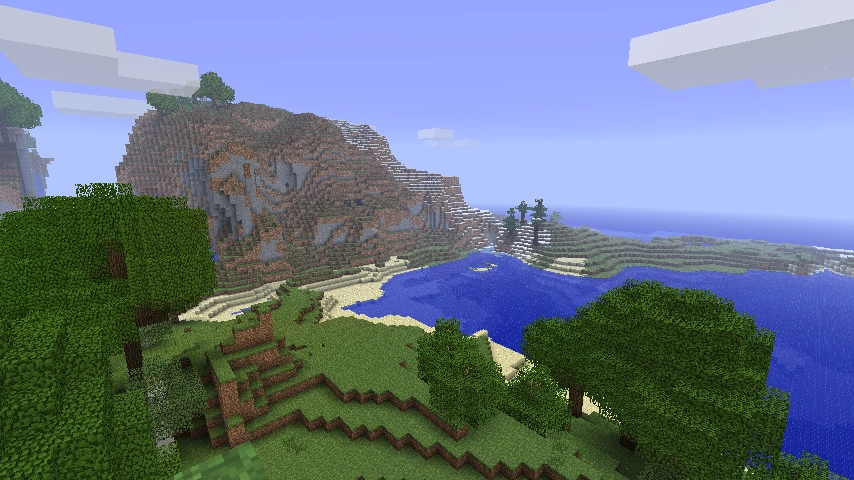
\includegraphics[width=0.8\textwidth]{figures/minecraft.png}
    \end{center}
    \caption{Screenshot from the game Minecraft, showing a voxel world rendered using polygon-based rendering. Source: Minecraft Wiki}
    \label{fig:minecraft}
\end{figure}

There are several techniques to produce a polygon mesh from a voxel grid, two popular techniques are Greedy Meshing (see
Section~\ref{sec:greedy_meshing}) and Marching Cubes.

\subsection{Greedy Meshing} \label{sec:greedy_meshing}
The naive approach to producing a mesh from a voxel grid is to iterate over each voxel, and for each voxel that isn't
empty, create a quad consisting of two triangles for each face that is adjacent to an empty voxel. This approach is simple
to implement, but produces a large number of triangles. Greedy meshing is an optimization to this approach that reduces
the number of triangles produced by merging identical adjacent voxels into a single quad. The two approaches can be seen
in Figure~\ref{fig:greedy_meshing}. Reducing the number of triangles can improve rendering performance as the GPU will have
fewer triangles to rasterize; similarly there will be less vertex data that needs to be transferred to the GPU.

\begin{figure}[thp]
    \begin{center}
        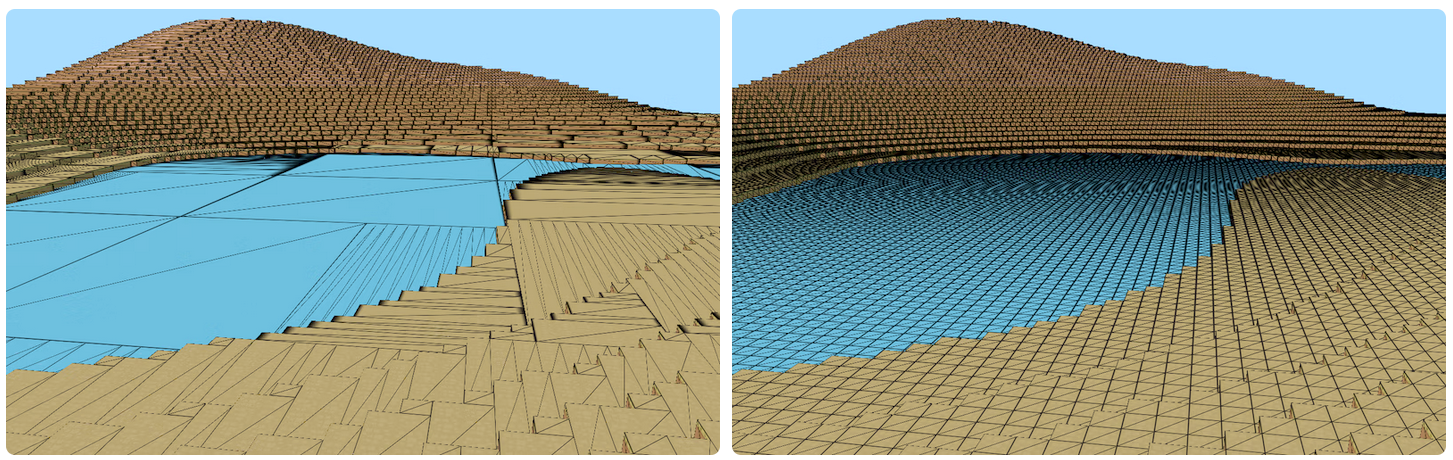
\includegraphics[width=0.8\textwidth]{figures/greedy_meshing.png}
    \end{center}
    \caption{Comparison of a voxel grid meshed using the naive approach (right) and greedy meshing (left).
        Source: Jason Gedge~\protect\cite{Gedge_2014}}
    \label{fig:greedy_meshing}
\end{figure}

\section{Ray Tracing}
Ray tracing is a rendering technique that simulates the way light interacts with objects in a scene. Rays are cast from the
camera, and for each pixel, the ray is traced through the scene to determine the color of the pixel (see Figure~\ref{fig:ray_tracing}).
Ray tracing is well suited to voxel rendering due to the volumetric nature of voxels, and other optimisations such as
bounding volume hierarchies (see Section~\ref{sec:bvh} and Section~\ref{sec:svo}). There are other advantages to using ray
tracing for voxel rendering, such as the ability to directly operate on the voxel data providing more flexibility in the
rendering process, instead of having to go through the intermediate step of converting voxels to triangles for rasterization.

\begin{figure}[thp]
    \begin{center}
        \scalebox{0.7}{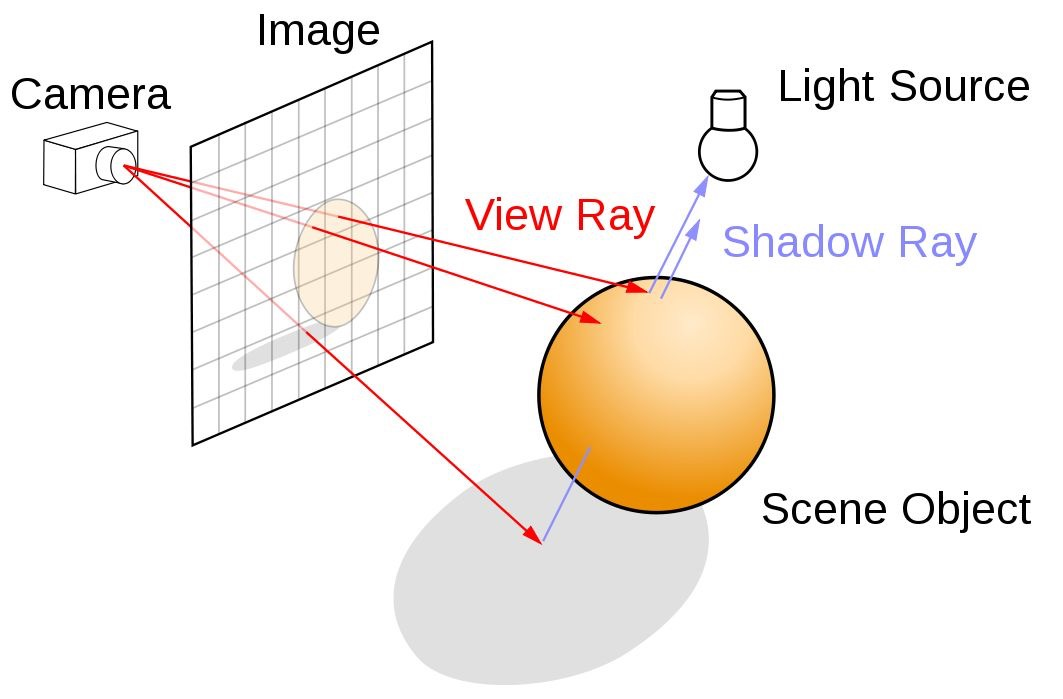
\includegraphics[width=0.8\textwidth]{figures/ray_tracing.jpg}}
    \end{center}
    \caption{Illustration of the ray tracing process. Rays are cast from the camera, and for each pixel, the ray is traced
        through the scene to determine the color of the pixel. Source: NVIDIA Developer}
    \label{fig:ray_tracing}
\end{figure}

\subsection{Digital Differential Analysis} \label{sec:dda}
Due to the nature of voxel grids, the ray tracing process can be simplified by using Digital Differential Analysis (DDA).
DDA is a line drawing algorithm that is used to traverse a grid, and can be adapted for ray tracing by stepping through the
voxel grid along the ray using pre-calculated intervals~\cite{Amanatides_Woo_1987}. Calculating the steps the ray takes
through the grid before hand saves time during the ray tracing process, and can be used to determine the intersection
points of the ray with the voxels. See Figure~\ref{fig:dda}.

\begin{figure}[thp]
    \begin{center}
        \scalebox{0.7}{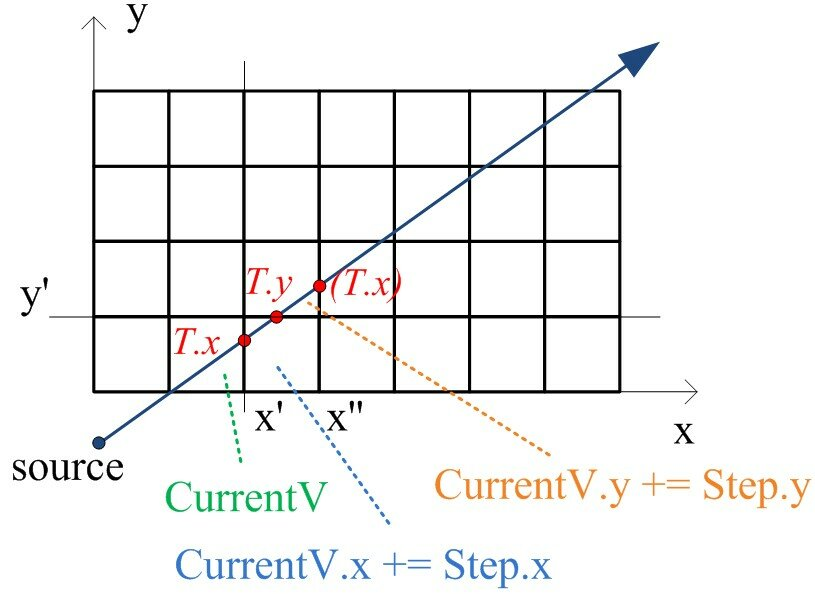
\includegraphics[width=0.8\textwidth]{figures/dda.jpg}}
    \end{center}
    \caption{A 2D example of the DDA algorithm. Steps values for the $x$ and $y$ axes are calculated before hand, and used
        to traverse the grid. Source:~\protect\cite{Xiao_2015}}
    \label{fig:dda}
\end{figure}

\subsection{Bounding Volume Hierachies} \label{sec:bvh}
Intersection tests are an important part of the ray tracing process, and can be computationally expensive. Bounding Volume
Hierarchies (BVHs) are a data structure that can be used to speed up the intersection tests by providing a way to quickly
determine which objects in the scene the ray intersects with~\cite{Ize_2009}. See Figure~\ref{fig:bvh}.

\begin{figure}[thp]
    \begin{center}
        \scalebox{0.8}{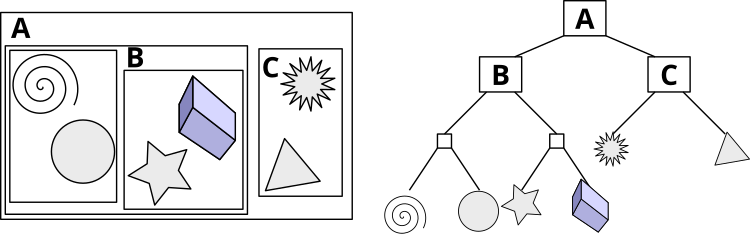
\includegraphics[width=0.8\textwidth]{figures/bvh.png}}
    \end{center}
    \caption{An example of a bounding volume hierarchy using rectangles as bounding volumes. Source: Wikipedia}
    \label{fig:bvh}
\end{figure}

A natural way to create a BVH for a voxel scene is to use an octree structure (see Section~\ref{sec:svo}), where each node
in the tree represents a bounding box that contains the voxels in the scene. The octree can be traversed to determine which
voxels the ray intersects with, and can be used to quickly determine the intersection points of the ray with the voxels
using the DDA algorithm (see Section~\ref{sec:dda}).

\section{Sparse Voxel Octrees} \label{sec:svo}
Sparse Voxel Octrees (SVOs) are a popular data structure for representing voxel scenes, as they provide a compact representation
of the scene by storing only the occupied voxels in a tree structure. Each node in the tree can be subdivided further into
8 children to achieve a desired resolution of the scene; this property also makes it easy to introduce LOD by only ray tracing
up to a specific depth in the tree. See Figure~\ref{fig:octree}.

\begin{figure}[thp]
    \begin{center}
        \scalebox{0.8}{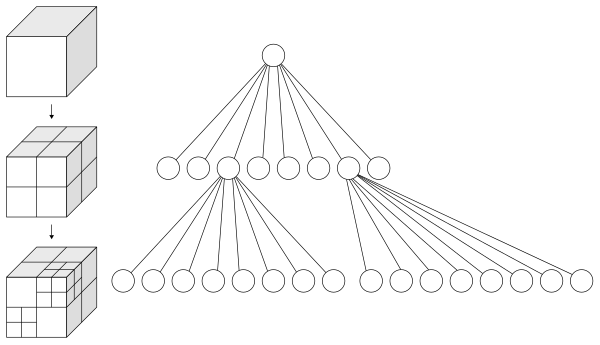
\includegraphics[width=0.8\textwidth]{figures/octree.png}}
    \end{center}
    \caption{Illustration of a voxel grid represented as a sparse voxel octree. Left: Recursive subdivision of a Cubes
        into octants. Right: The corresponding octree. Source: Wikipedia}
    \label{fig:octree}
\end{figure}

Octrees are most easily implemented using pointers which works well on the CPU, but can be inefficient on the GPU due to
the lack of support for pointers. To address this, SVOs are usually further compressed into a format better suited for the
GPU such as a 1D array, using techniques such as run-length encoding (RLE)~\cite{Eisenwave_RLE} and space filling curves
(SFC)~\cite{Eisenwave_SFC}.

\subsection{Space Filling Curves}
Space Filling Curves (SFCs) are a way of mapping a 2D or 3D space into a 1D space, and are used to linearize the octree
structure of an SVO into an array. SFCs can provide better cache locality when traversing the octree, as neighbouring
voxels in 3D space are likely to be close together in the 1D array. A popular SFC used in voxel rendering is the Morton
code, also known as the Z-order curve. See Figures~\ref{fig:morton} and~\ref{fig:morton_3d}.

\begin{figure}[thp]
    \begin{center}
        \scalebox{0.8}{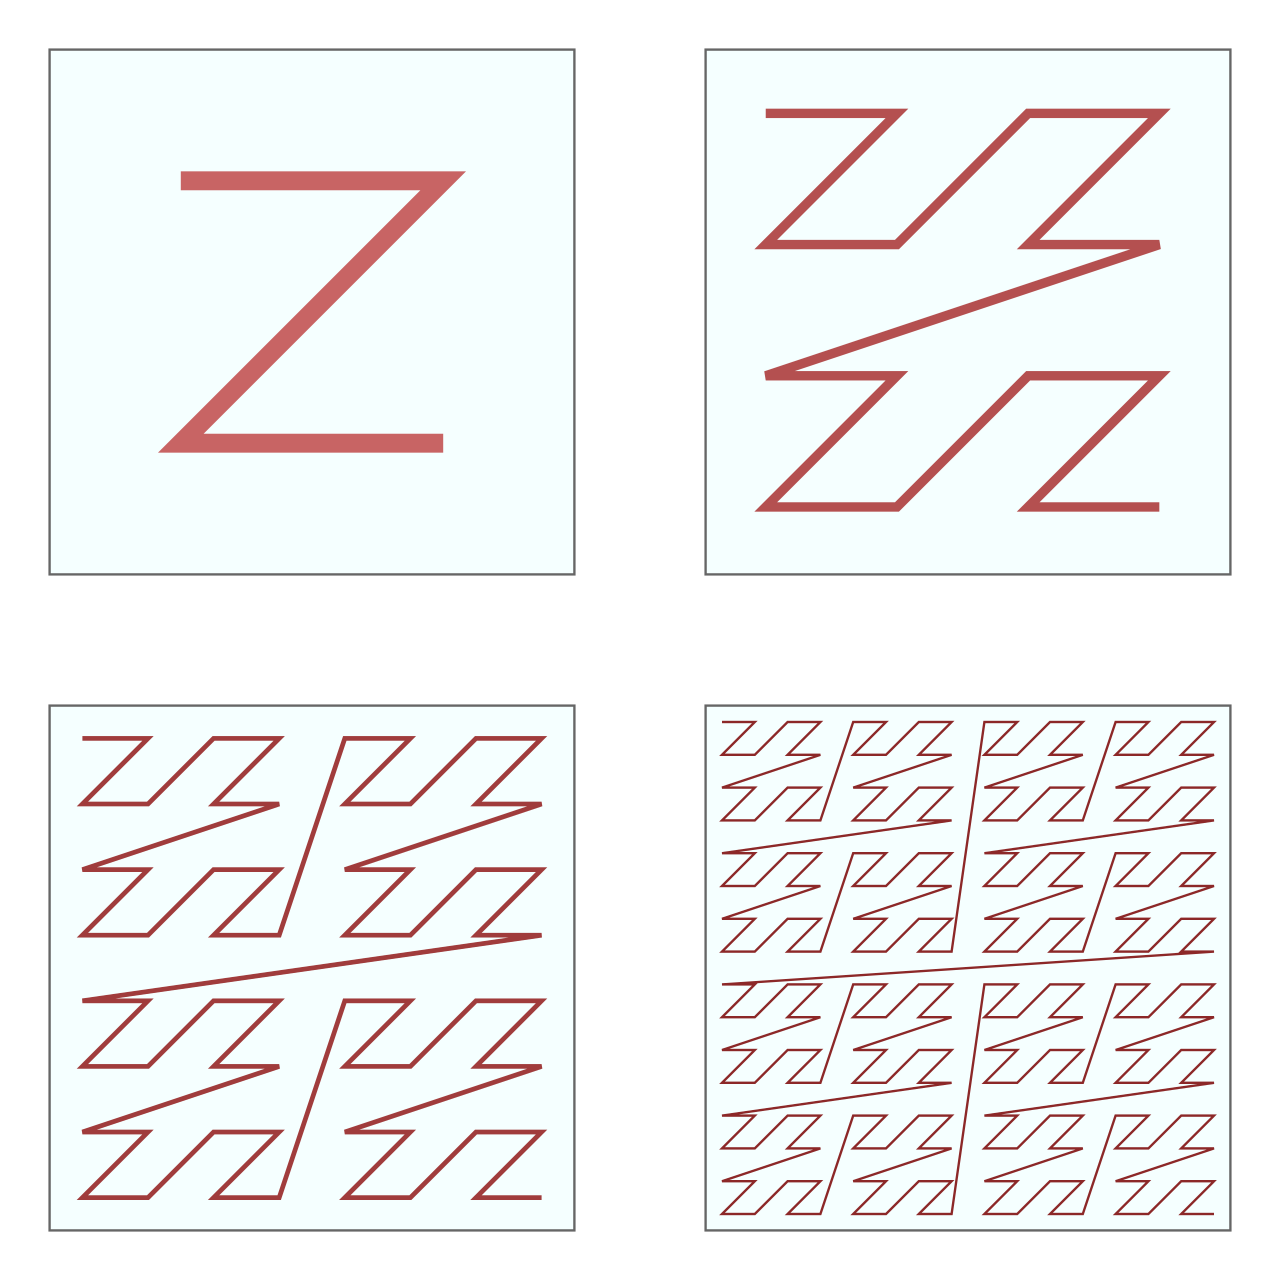
\includegraphics[width=0.8\textwidth]{figures/morton.png}}
    \end{center}
    \caption{Four iterations of the Z-order curve (Morton code) on a 2D grid. Source: Wikipedia}
    \label{fig:morton}
\end{figure}

\begin{figure}[thp]
    \begin{center}
        \scalebox{0.8}{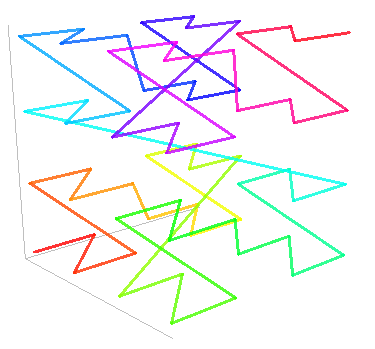
\includegraphics[width=0.8\textwidth]{figures/morton_3d.png}}
    \end{center}
    \caption{Extension of the Z-order curve (Morton code) to 3D space. Source: Wikipedia}
    \label{fig:morton_3d}
\end{figure}

\subsection{Sparse Voxel Directed Acyclic Graphs}
SVOs can be further optimized by using Sparse Voxel Directed Acyclic Graphs (SVDAGs)~\cite{Kampe_Sintorn_Assarsson_2013}.
SVDAGs are a way of further compressing an SVO by removing redundant nodes in the tree that contain identical nodes. This
can lead to being able to store larger scenes in memory (in the billions of voxels~\cite{Kampe_Sintorn_Assarsson_2013})
while still maintaining a low memory footprint. In the context of the dissertation, this technique could be used to store
the voxel data on the GPU in a more compact format, and reduce the amount of data that needs to be transferred between the
host and device; however, updating an SVDAG can be more complex than updating an SVO which would not be suited to dynamic updates.

\section{Dynamic Updates}
Updating an SVO can be a straightforward process as only the affected nodes need updating; however, updating a compressed
format, and transferring the new data to the GPU, can be computationally expensive~\cite{Crassin_2012}. A common approach
is to divide a voxel scene into a dynamic and static SVO~\cite{Douglas_2022,Pan_2021}.

There are several approaches for merging two octrees together, each of which are suited to different scenarios such as
addition or removal of voxels. The two common algorithms are Jessup's and Pham's algorithms~\cite{Jessup_2014,Pham_2007}.